\documentclass{erciyes}

\usepackage{graphicx}
\usepackage{amsmath}
\usepackage{amssymb}
\usepackage{booktabs}
\usepackage{tabularx}
\usepackage{array}
\usepackage{float}
\usepackage{xcolor}
\usepackage{listings}
\usepackage{cite}

\renewcommand{\thetable}{\arabic{table}}   % bölüm numarası kullanılmadığı için
\renewcommand{\thefigure}{\arabic{figure}}

% Türkçe kelimeler uzun olduğu için satırlar taşabiliyor;
% bu ayar kelimeler arasındaki boşluğu biraz esnetip taşmayı azaltıyor.
\setlength{\emergencystretch}{3em}

\ToCLineisDotted %% İçindekiler kısmında sayfa numaralarına kadar olan kısım noktalı olsun
\ToCChapterBold  %% İçindekiler kısmında BÖLÜM 1-2... yazıları bold olsun.
%\TabloListesiYok %% Tablo Listesi kullanılmayacak
%\SekilListesiYok %% Şekil Listesi kullanılmayacak

\setlength{\fboxsep}{0pt}

\newcommand{\plotPGFfile}{true} % PGF olarak DATA dosyaları çizilsin mi çizilmesin mi? Çizilmez ise dosyadan sadece data okunan kısım atlanıyor, resmin çerçevesi oluşturuluyor...
\definecolor{dkgreen}{rgb}{0,0.6,0}
\definecolor{gray}{rgb}{0.5,0.5,0.5}
\definecolor{mauve}{rgb}{0.58,0,0.82}

\lstset{frame=tb,
	language=Java, %Uygulamanın yazıldığı programlama dili, (Örnek kullanım chapter4.tex'te verilmiştir.)
	aboveskip=3mm,
	belowskip=3mm,
	showstringspaces=false,
	columns=flexible,
	basicstyle={\small\ttfamily},
	numbers=none,
	numberstyle=\tiny\color{gray},
	keywordstyle=\color{blue},
	commentstyle=\color{dkgreen},
	stringstyle=\color{mauve},
	breaklines=true,
	breakatwhitespace=true,
	tabsize=3
}

\author{Mustafa}{G{\"O}KTEPE}{1030510749}{1030510749@erciyes.edu.tr}{05331556738}%1. Öğrenci ad soyad
\authorIki{Ahmet}{ÇELİK}{1030510691}{1030510691@erciyes.edu.tr}{05453246440}%2. Öğrenci ad soyad Opsiyonel
\authorUc{Mustafa}{KÜPELİ}{1030510266}{1030510266@erciyes.edu.tr}{05360100620}%3. Öğrenci ad soyad  Opsiyonel
%\authorDort{Ad}{Soyad}{103051004}{numara4@erciyes.edu.tr}{054xxxxxxx}%4. Öğrenci ad soyad Opsiyonel

\anabilimdali{Bilgisayar Mühendisliği}
\anabilimdaliUpper{BİLGİSAYAR MÜHENDİSLİĞİ}

\date{Kasım 2026}
\Yil{2026-2027} %Eğitim Öğretim Yili
\Donem{Güz} %Donemi
\teziyoneten{Ar.\ G{\"O}r. HAYRİ ÖZTÜRK} % Tez Danismani





\title{MEDIAPIPE VE MAKİNE ÖĞRENMESİ KULLANARAK TÜRK İŞARET DİLİ (TİD) TABANLI GERÇEK ZAMANLI EL HAREKETİ TANIMA VE ÇEVİRİ SİSTEMİ} %TAMAMEN BÜYÜK HARF\vspace*{5mm}
\titleCase{MediaPipe ve Makine Öğrenmesi Kullanarak Türk İşaret Dili (TİD) Tabanlı Gerçek Zamanlı El Hareketi Tanıma ve Çeviri Sistemi} %Sadece ilk Harfleri Büyük




\renewcommand{\textfraction}{0.10}
\renewcommand{\topfraction}{0.95}
\renewcommand{\bottomfraction}{0.95}
\renewcommand{\floatpagefraction}{0.35}

\setcounter{totalnumber}{5}

\begin{document}
\clearpage
\section{Özet}
\label{CH:BolumOzet}

Bu projede, işitme ve konuşma engelli bireylerin günlük iletişimde karşılaştığı
sorunları azaltmak amacıyla akıllı telefon kamerasından alınan Türk İşaret Dili
(TİD) hareketlerini tanıyıp yazıya çeviren bir sistem geliştirilmektedir. Sistem,
işareti video olarak kaydedip bir sunucuya göndermek yerine telefonda çıkarılan
iskelet koordinatları üzerinde çalışmaktadır. Böylece internet bağlantısına ihtiyaç
kalmamakta, kamera görüntüsü de cihazdan dışarı çıkmamaktadır.

Veri tarafında AUTSL veri setinin resmî \texttt{train}, \texttt{val} ve
\texttt{test} bölmeleri kullanılmıştır. Bölmeler arasında işaretçi kesişmediği
doğrulanmış, açılamayan 11 video tespit edilerek çıkarım dışında bırakılmıştır.
Her karede iki elin 21'er noktası ve üst gövdeye ait 7 nokta Google MediaPipe
Tasks API ile çıkarılmıştır. Koordinatlar omuz ortasına göre ötelenmiş ve omuz
genişliğine bölünmüş, değişken uzunluktaki diziler 64 kareye örneklenmiştir.

Sınıflandırma aşamasında PyTorch ile iki katmanlı, iki yönlü bir GRU (BiGRU)
temel modeli ve karşılaştırma amacıyla üç katmanlı 1B-CNN + iki katmanlı
Transformer modeli kurulmuştur. Aynı veri ve artırma düzeninde 60 epoch sonunda
BiGRU modeli test kümesinde yüzde 88,24 (doğrulama yüzde 89,23), daha hafif olan
1B-CNN + Transformer modeli ise yüzde 88,83 (doğrulama yüzde 89,97) Top-1
doğruluğa ulaşarak tez önerisindeki yüzde 85 hedefini aşmıştır. Temel modelin
LiteRT int8 sürümü 3,19 MB boyutundadır ve aynı 200 test örneği Python ile
telefon üzerinde çalıştırıldığında tahminlerin yüzde 99,5'i birbiriyle aynı
çıkmıştır.

Mobil tarafta Kotlin/CameraX ile kurulan kamera ve çıkarım hattı Flutter
arayüzüne bağlanmıştır. Telefonda model çıkarımı ortalama 48 ms sürmektedir.
Buna karşılık kamera, MediaPipe ve arayüz dâhil uçtan uca hız yaklaşık 9 FPS'tir
ve hedeflenen 15 FPS'in altında kalmaktadır. Canlı kamera kullanımında tahmin
güvenlerinin kaydedilmiş veriye göre belirgin biçimde düştüğü gözlenmiş, nedeni
henüz kesinleştirilememiştir. Bu iki konu sonuç bölümünde ayrıca tartışılmaktadır.

\clearpage
 %Özet
\section{Motivasyon}
\label{IkinciBolum}

Türk İşaret Dili, işitme engelli bireylerin hem kendi aralarında hem de
çevreleriyle iletişim kurarken kullandığı doğal dildir~\cite{TIF2023}. Ancak
işaret dilini bilmeyen kişilerle kurulan iletişim çoğu zaman yazı yazmaya ya da
bir yakının tercümanlığına bağlı kalmaktadır. Hastane, banka, okul ve resmî
daire gibi ortamlarda bu durum hem zaman kaybına hem de ciddi bir mahremiyet
sorununa yol açmaktadır.

Projenin çıkış noktası, bu iletişim barındaki en yaygın cihazı kullanmaktır.
Eldiven, derinlik kamerası gibi ek donanım gerektirmeyen bir çözüm, kullanıcı
açısından kabul edilebilirliği artırır ve maliyeti düşürür. Bu nedenle sistem
yalnızca telefon kamerası ve cihaz üzerinde çalışan bir model ile kurgulanmıştır.
İnternet bağlantısına ihtiyaç duymaması, uygulamanın sınıfta, hastanede veya
şebekenin zayıf olduğu yerlerde de kullanılabilmesini sağlar.

Beklenen katkı, kelime düzeyinde çalışan bir tanıma modülünün mobil cihazda
gerçek zamanlıya yakın hızda çalıştığını göstermektir. Cümle çevirisi projenin
kapsamı dışında bırakılmış ve gelecek çalışma olarak not edilmiştir.

Çalışma üç sorumluluk alanına ayrılmıştır: mobil uygulama, kullanıcı arayüzü ve
donanım entegrasyonu (Ahmet Çelik); yapay zekâ modeli, eğitim ve optimizasyon
(Mustafa Göktepe); veri hazırlığı, veri hattı ve normalizasyon (Mustafa Küpeli).
Bu raporun yöntem bölümü ağırlıklı olarak model tarafını anlatmaktadır.
 %Motivasyon
\section{Projenin İçerdiği Yenilik Unsuru}
\label{UcuncuBolum}

Literatürdeki çalışmaların önemli bir kısmı yabancı işaret dilleri (ASL, BSL vb.)
üzerinedir ve genellikle sunucu tarafında çalışan büyük modeller kullanır. Bu
proje doğrudan TİD üzerine kurulmuştur ve AUTSL'nin resmî bölmelerini kullanarak
tekrarlanabilir bir değerlendirme düzeni oluşturur~\cite{AUTSL2020}. Kullanılan
bölmelerde işaretçi kesişmesi bulunmadığı için elde edilen doğruluk, modelin daha
önce görmediği kişiler üzerinden ölçülmüş olur.

Yenilik iddiası modelin kendisinden çok, hattın uçtan uca ve telefonda
çalışmasındadır. Şu üç nokta öne çıkmaktadır:

\begin{itemize}
  \item Girdi olarak video karesi değil iskelet koordinatları kullanılmıştır.
        Model 2,1 milyon parametreyle sınırlı kaldığı için 10 MB'lık boyut hedefi
        rahatça sağlanmış, ayrıca ham görüntü işlenmediği için kişisel veri yükü
        azalmıştır.
  \item Nokta çıkarımı hem eğitim hem uygulama tarafında aynı MediaPipe Tasks API
        ile yapılmıştır. Bu, iki taraf arasındaki nokta sıralaması ve
        normalizasyon farkından doğabilecek hataları büyük ölçüde ortadan
        kaldırmıştır. Dönüşüm sonrası Python ve LiteRT çıktılarının yüzde 99,5
        oranında aynı olması bunu desteklemektedir.
  \item Sistem tamamen çevrimdışı çalışmaktadır; model dosyası uygulamanın içinde
        taşınmakta ve çıkarım cihazda yapılmaktadır.
\end{itemize}
 %Projenin İçerdiği Yenilik Unsuru
\section{Yöntem ve Metotlar}
\label{DorduncuBolum}

Projenin ilk dikey dilimi veri hazırlığı, nokta çıkarımı, model eğitimi ve mobil
dönüşüm olmak üzere dört adımda tamamlanmıştır. Bu bölümde sırasıyla veri seti,
ön işleme, model mimarisi, eğitim düzeni ve değerlendirme anlatılmaktadır.

\subsection{Veri seti}

Çalışmada AUTSL veri seti kullanılmıştır~\cite{AUTSL2020}. Veri setinde 226
işaret, 43 işaretçi ve toplam 36.302 video bulunmaktadır. Resmî bölmeler
\texttt{train} (28.142), \texttt{val} (4.418) ve \texttt{test} (3.742) şeklindedir.
Bölmelerin işaretçi bazında ayrık olduğu, sınıf numaralarının üç bölmede de aynı
anlama geldiği ayrıca kontrol edilmiştir.

Kaggle üzerinden indirilen kopyada 11 videonun açılamadığı görülmüştür. Bu
dosyalarda MP4 kutusuna ait \texttt{moov} bilgisi eksiktir, yani dosyalar yarım
inmiştir. İlgili videolar çıkarım sırasında atlanmış, kalan 28.132 train, 4.418
val ve 3.741 test videosu ile çalışılmıştır. Atlanan dosyaların listesi depodaki
\texttt{docs/data.md} dosyasında tutulmaktadır. Sınıf numarası ile Türkçe kelime
eşlemesi \texttt{SignList\_ClassId\_TR\_EN.csv} dosyasından okunmaktadır.

\subsection{Nokta çıkarımı ve normalizasyon}

Her video karesi MediaPipe Tasks API'ye verilmiş, iki el için 21'er nokta ve üst
gövde için 7 nokta (burun, iki omuz, iki dirsek, iki bilek) alınmıştır~\cite{MediaPipe2019}.
El modeli olarak \texttt{hand\_landmarker}, gövde modeli olarak
\texttt{pose\_landmarker\_lite} kullanılmıştır. Çıkarım sonucunda ellerin bulunma
oranı sol elde yüzde 82, sağ elde yüzde 86 olarak ölçülmüştür; gövde noktaları tüm
karelerde yakalanmıştır. Elin bulunmadığı karelerde ilgili koordinatlar
sıfırlanmakta, ayrıca iki boyutlu bir \sol el var mı\sag{} göstergesi özellik
vektörüne eklenmektedir.

Normalizasyon iki adımdan oluşmaktadır. Önce tüm noktalar iki omzun orta noktasına
göre ötelenir, ardından omuz genişliğine bölünür. Böylece kameraya olan uzaklık ve
kişinin boyu modeli etkilemez. Omuz noktasının bulunamadığı karelerde bir önceki
geçerli değer taşınmıştır. Normalizasyondan sonra her kare
$2\times21\times2 + 7\times2 + 2 = 100$ boyutlu bir vektörle temsil edilmektedir
(koordinatlar $x$ ve $y$; derinlik bilgisi kullanılmamıştır). Değişken
uzunluktaki diziler eğitim sırasında 64 kareye doğrusal interpolasyonla
örneklenmektedir.

\subsection{Model mimarisi}

Sınıflandırıcı olarak iki katmanlı ve iki yönlü bir GRU (BiGRU) kurulmuştur.
Girdi önce 100 boyuttan 256 boyuta indirgenir (doğrusal katman, ReLU, yüzde 20
dropout). Ardından iki GRU katmanı ileri ve geri yönde çalışır. Çıkışta son gizli
durum yerine zaman ekseni boyunca ortalama alınır; işaretin tamamı tek bir vektöre
indirildikten sonra 226 sınıfa yönelik doğrusal katman uygulanır. Zaman
ortalamasının seçilme nedeni, işaretin hangi karede bittiğinin kesin olmaması ve
dizinin başındaki ya da sonundaki boş karelerin sonucu kaydırmasının
istenmemesidir. Modelin parametre dağılımı Tablo~\ref{tab:model} içinde
verilmiştir.

\begin{table}[H]
\centering
\caption{BiGRU modelinin katmanları ve parametre sayıları}
\label{tab:model}
\begin{tabular}{lrr}
\toprule
\textbf{Katman} & \textbf{Çıkış boyutu} & \textbf{Parametre} \\
\midrule
Girdi doğrusal katmanı & $T\times256$ & 25.856 \\
GRU katmanı 1 (iki yönlü) & $T\times512$ & 787.968 \\
GRU katmanı 2 (iki yönlü) & $T\times512$ & 1.181.184 \\
Çıkış doğrusal katmanı & 226 & 115.938 \\
\midrule
\textbf{Toplam} & & \textbf{2.114.018} \\
\bottomrule
\end{tabular}
\end{table}

Karşılaştırma amacıyla ikinci bir mimari olarak üç katmanlı 1B evrişim ağı
(1D-CNN) ile iki katmanlı Transformer kodlayıcısının birleşiminden oluşan
\texttt{CNNTransformerNet} kurulmuştur. Evrişim katmanları
($100\rightarrow 128\rightarrow 256\rightarrow 256$)
kısa süreli yerel el hareketlerini çıkarırken, ikinci katmandaki $\text{stride}=2$
adımı dizi uzunluğunu $T=64$'ten $32$'ye indirerek sonraki dikkat (attention)
hesabının maliyetini yarıya düşürmektedir. Sinüzoidal konum kodlamasının ardından
gelen 2 katmanlı Transformer kodlayıcısı ($d_{\text{model}}=256$, 4 kafa,
ileri-besleme boyutu 512, GELU) uzun menzilli zaman ilişkilerini öğrenmektedir.
Bu model toplam 1.467.618 parametreye sahiptir (BiGRU'dan yaklaşık yüzde 30 daha
küçük) ve tekrarlayan katman içermediği için GPU/MPS üzerinde çok daha hızlı
eğitilebilmektedir.

\subsection{Eğitim düzeni}

Her iki model de PyTorch ile aynı veri, aynı artırma ve aynı hiperparametrelerle
eğitilmiştir: 60 epoch, AdamW optimizasyonu ($\text{lr}=2\times10^{-3}$, weight
decay $10^{-2}$), kosinüs öğrenme oranı azaltımı, 128'lik batch ve 0,1 etiket
yumuşatma. Doğrulama doğruluğu en yüksek olan epoch'un ağırlıkları saklanmış,
test kümesi yalnızca eğitim bittikten sonra bir kez ölçülmüştür. Apple M4 (MPS)
üzerinde 60 epoch'luk eğitim BiGRU için 77,6 dakika, tekrarlayan katman
içermeyen 1B-CNN + Transformer için ise yalnızca 18,1 dakika sürmüştür.

Eğitimde dört tür artırma uygulanmaktadır. Bunlardan en önemlisi zamansal
seyreltmedir: video kareleri rastgele 1, 2 veya 3 adımda bir örneklenerek 30, 15
veya 10 FPS'lik kayıtlara benzetilir. Bu artırmanın nedeni, telefon kamerasının
gerçek kullanımda yaklaşık 9--10 FPS civarında kare üretmesi ve modelin bu
koşulda da çalışması gerektiğidir. Diğer artırmalar dizinin iki ucundan yüzde
10'a kadar kırpma, $\pm10^\circ$ döndürme ve yüzde 90--110 arası ölçek
değişimidir. Artırma yalnızca eğitim kümesine uygulanmaktadır.

\subsection{Değerlendirme ve hata analizi}

Sonuçlar 226 sınıf üzerinde Top-1 doğruluk ve sınıf bazlı Macro F1 ile
ölçülmüştür. İki mimarinin aynı tohum (\texttt{seed=0}) ve 60 epoch altındaki
karşılaştırması Tablo~\ref{tab:karsilastirma} içinde, epoch bazındaki eğitim
kaybı ve doğrulama doğruluğu eğrileri ise Şekil~\ref{fig:egri} üzerinde
gösterilmiştir.

\begin{table}[H]
\centering
\caption{226 sınıfta BiGRU ve 1B-CNN + Transformer karşılaştırması (60 epoch)}
\label{tab:karsilastirma}
\small
\setlength{\tabcolsep}{3.5pt}
\begin{tabular}{@{}lrrrrr@{}}
\toprule
\textbf{Model} & \textbf{Parametre} & \textbf{Val (\%)} & \textbf{Test (\%)} & \textbf{F1 (\%)} & \textbf{Süre (dk)} \\
\midrule
BiGRU-2x256 & 2.114.018 & 89,25 & 88,24 & 88,09 & 77,6 \\
1B-CNN + Transformer & 1.467.618 & \textbf{90,02} & \textbf{88,83} & \textbf{88,61} & \textbf{18,1} \\
\bottomrule
\end{tabular}
\end{table}

\begin{figure}[H]
\centering
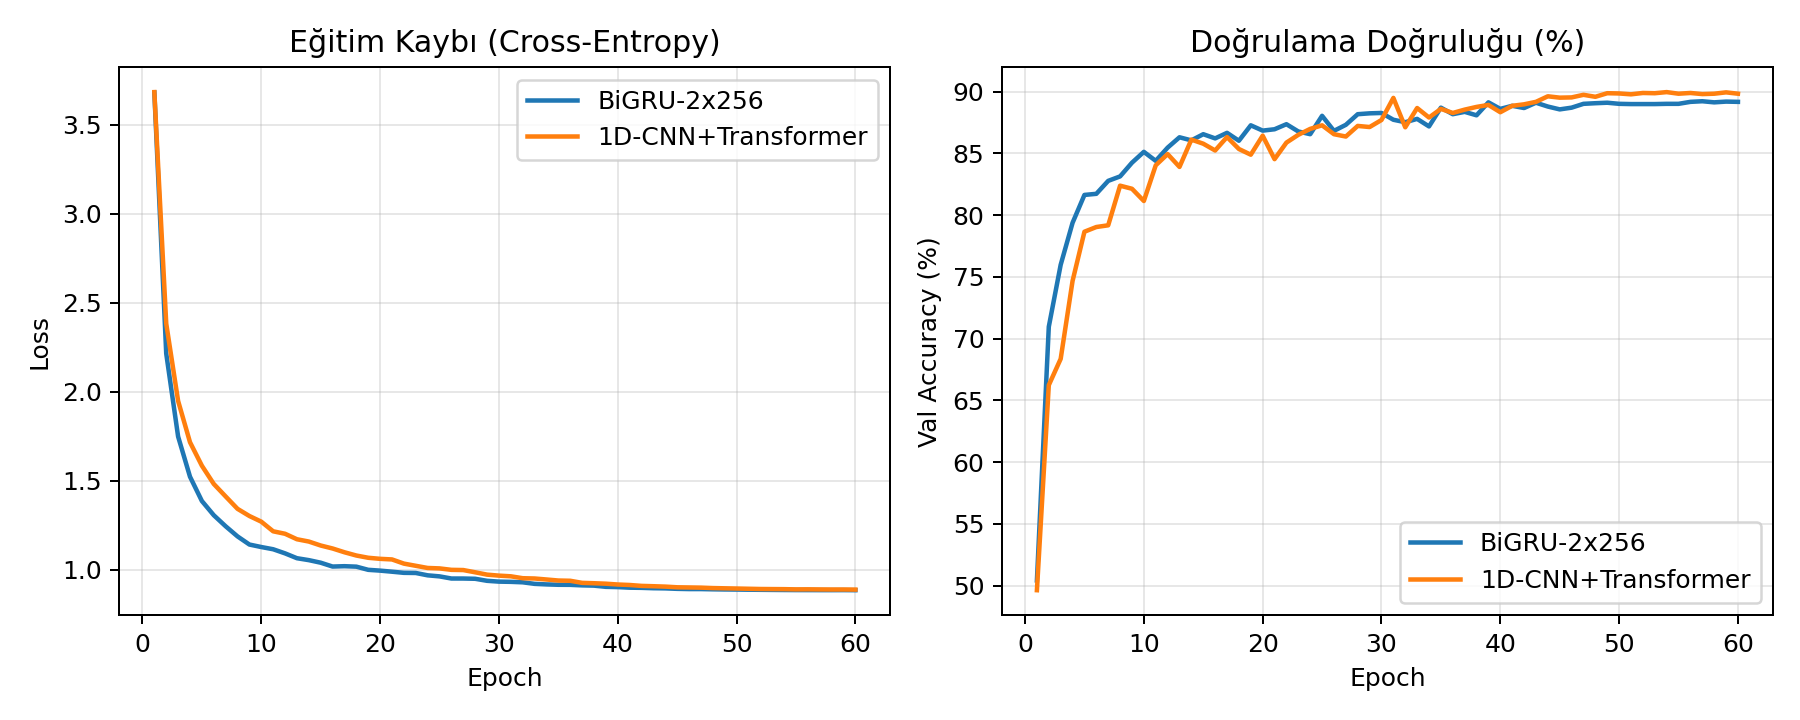
\includegraphics[width=0.95\textwidth]{grafik/egitim_egrisi.png}
\caption{BiGRU-2x256 ve 1B-CNN + Transformer modellerinin 60 epoch boyunca eğitim kaybı ve doğrulama doğruluğu eğrileri}
\label{fig:egri}
\end{figure}

Şekil~\ref{fig:egri} incelendiğinde BiGRU modelinin ilk 15 epoch'ta daha hızlı
yükseldiği, ancak 30. epoch sonrasında 1B-CNN + Transformer modelinin öne geçerek
yüzde 90,02 doğrulama ve yüzde 88,83 test doğruluğuna ulaştığı görülmektedir.
Ayrıca önceki GPU koşusunda elde edilen BiGRU ağırlıkları da yüzde 89,9 doğrulama
ve yüzde 88,0 test doğruluğu ile aynı bandı teyit etmektedir.

Hata kaynaklarını anlamak için test kümesindeki 3.741 örnek üzerinde karışıklık
matrisi ve sınıf bazlı F1 skorları çıkarılmıştır. En çok birbiriyle karışan 18
sınıfın alt karışıklık matrisi Şekil~\ref{fig:cm} üzerinde, iki modelde en sık
görülen karışma çiftleri ise Tablo~\ref{tab:karisan} içinde verilmiştir.

\begin{figure}[H]
\centering
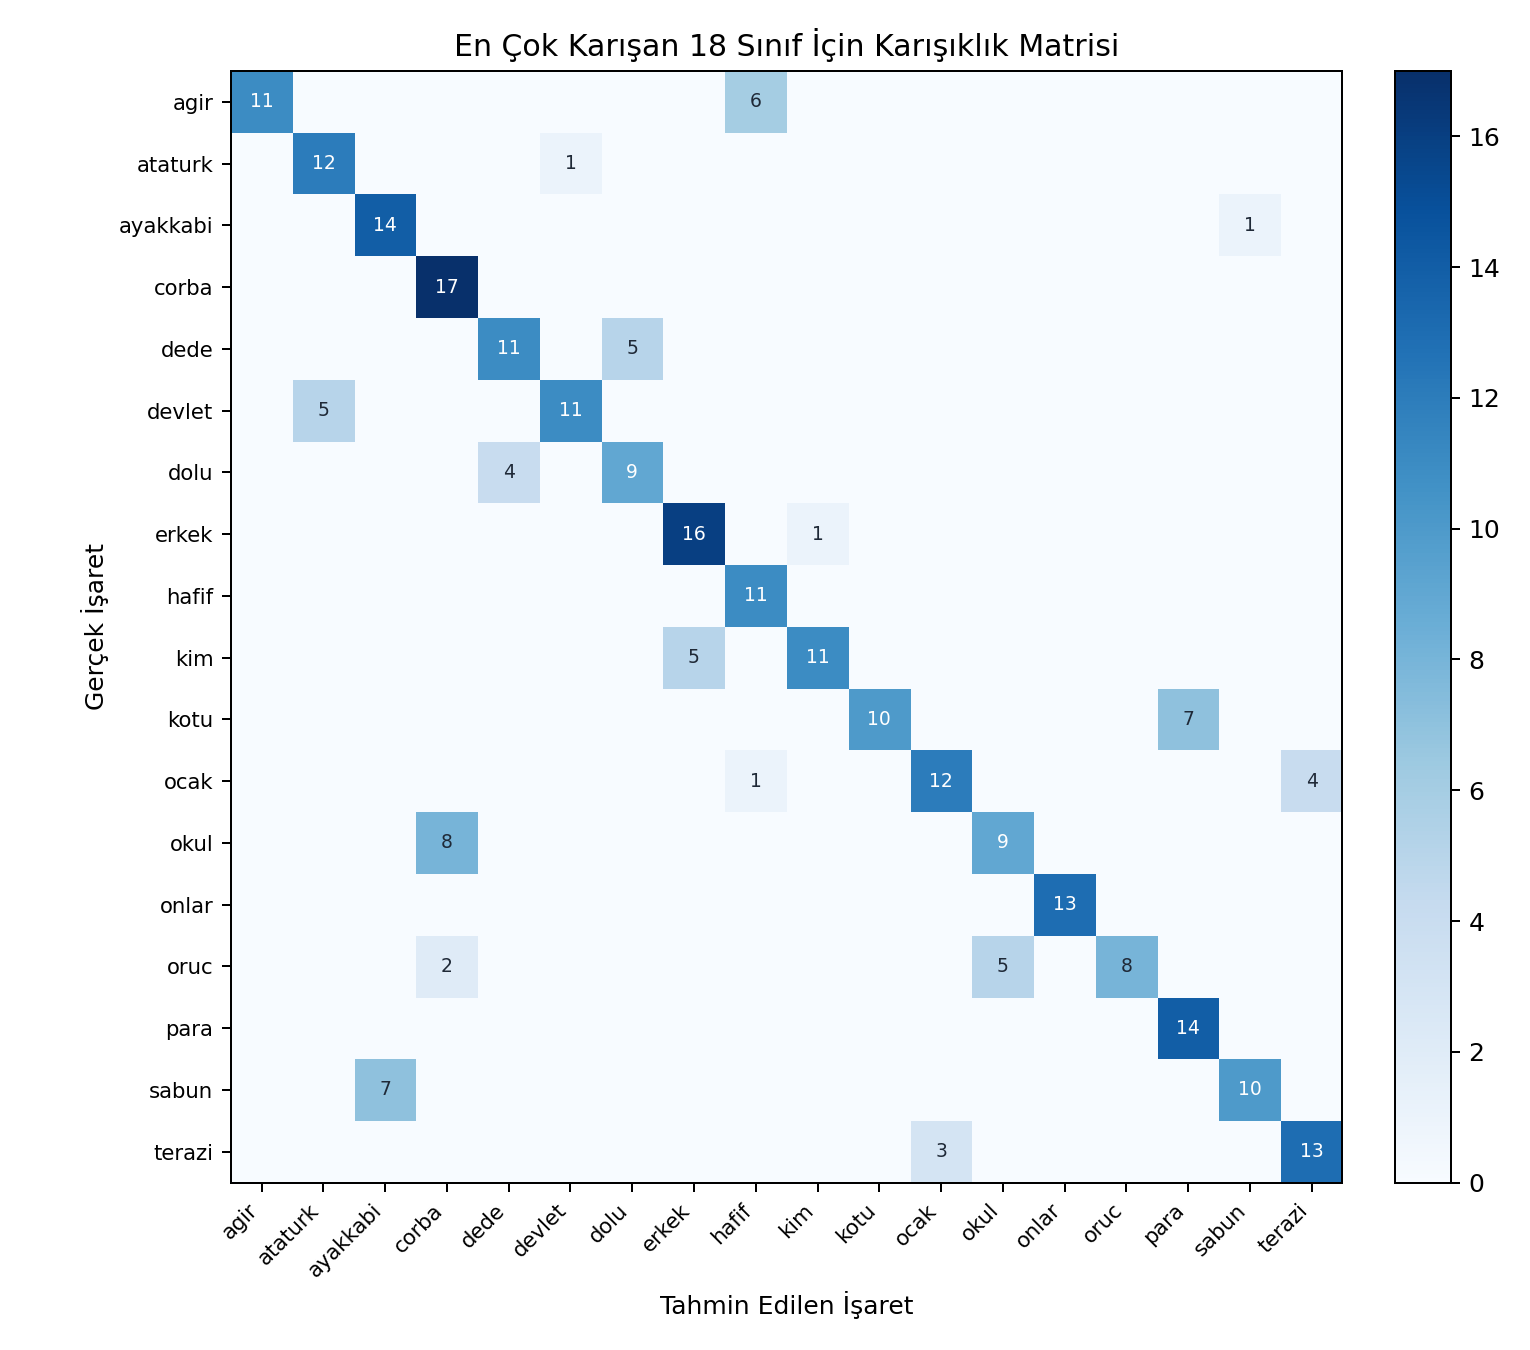
\includegraphics[width=0.88\textwidth]{grafik/karisiklik_matrisi.png}
\caption{Test kümesinde en çok karışan 18 sınıf için karışıklık matrisi (1B-CNN + Transformer)}
\label{fig:cm}
\end{figure}

\begin{table}[H]
\centering
\caption{Test kümesinde en sık birbiriyle karışan işaret çiftleri ve nedenleri}
\label{tab:karisan}
\small
\begin{tabularx}{\textwidth}{@{}l l r X@{}}
\toprule
\textbf{Gerçek İşaret} & \textbf{Tahmin Edilen} & \textbf{Hata / Toplam} & \textbf{Benzerlik Nedeni} \\
\midrule
okul (144) & çorba (43) & 8 / 17 & İki elin göğüs önünde benzer kavisli hareketi \\
kötü (122) & para (154) & 7 / 17 & Parmak ucu sürtme hareketinin 2B izdüşümde benzemesi \\
sabun (166) & ayakkabı (17) & 7 / 17 & İki elin birbirine sürtünme hareketi \\
ağır (6) & hafif (79) & 6 / 17 & Aynı iki el formu, yalnızca zıt yönlü (aşağı/yukarı) hareket \\
dede (48) & dolu (53) & 5 / 17 & Çene/ağız hizasında başlayan benzer el konumu \\
\bottomrule
\end{tabularx}
\end{table}

Tablo~\ref{tab:karisan} incelendiğinde hataların rastgele olmadığı, el formu ve
konumu aynı olup yalnızca ince parmak teması veya derinlik ekseninde ayrışan
işaretlerde toplandığı görülmektedir. Uygulamada sözlükte olmayan bir hareketin
yanlış sınıfa atanmasını engellemek için yapılan güven eşiği taramasında 0,6
eşiği seçilmiştir: bu eşiğin üzerinde kalan örnekler test kümesinin yaklaşık
yüzde 75'idir ve bu örneklerde doğruluk yüzde 96,8'e çıkmaktadır. Eşiğin altında
kalan tahminler arayüzde gösterilmemektedir.

\subsection{Mobil dönüşüm ve parite}

Eğitilen model önce NumPy ağırlıklarına aktarılmış, Keras üzerinden LiteRT
(\texttt{.tflite}) biçimine dönüştürülmüştür. Ardından dinamik aralık int8
nicemleme uygulanmıştır. Dosya boyutu fp32 sürümde 9,43 MB iken int8 sürümde
3,19 MB'a inmiştir; int8 modelin test doğruluğu yüzde 88,0 olarak aynı kalmıştır.

Dönüşümün doğru yapıldığını görmek için 200 test örneği hem Python hem telefon
üzerinde çalıştırılmış, tahminlerin yüzde 99,5'i aynı çıkmıştır. Telefonda model
çıkarımı ortalama 48 ms sürmektedir (Redmi Note 10 Pro). Ancak bu süre yalnızca
modeli kapsamaktadır. Kamera görüntüsünün alınması, MediaPipe ile el ve gövde
noktalarının çıkarılması ve arayüz güncellemesi de eklendiğinde uçtan uca hız
yaklaşık 9 FPS'e düşmektedir. Darboğaz model değil, kare başına iki ayrı MediaPipe
modelinin çalıştırılmasıdır.

Flutter arayüzü ile Kotlin tarafı arasındaki iletişim olay kanalları (event
channel) üzerinden kurulmuştur. Kamera, MediaPipe ve LiteRT işlemleri Kotlin
tarafında kalmakta, Flutter yalnızca ekranları ve durum bilgisini yönetmektedir.
 %Yöntem ve Metotlar
\section{Proje Planı}
\label{BesinciBolum}

Projenin kilometre taşları ve 3 Kasım 2026 itibarıyla durumları
Tablo~\ref{tab:plan} içinde verilmiştir. M1 kapsamındaki nokta çıkarımı, BiGRU ve
1B-CNN + Transformer modellerinin 60 epoch eğitimi, hata analizi ve LiteRT
dönüşümü tamamlanmış; çoklu tohum (seed) koşuları ve mobil uygulamanın kalan
ekranları M3 ve M4 altında planlanmıştır.

\begin{table}[H]
\centering
\caption{Kilometre taşları ve durumları}
\label{tab:plan}
\small
\begin{tabularx}{\textwidth}{@{}l l l X@{}}
\toprule
\textbf{Kilometre Taşı} & \textbf{Tarih} & \textbf{Durum} & \textbf{Çıktı / Açıklama} \\
\midrule
T1 & 5 Ekim 2026 & Tamamlandı & Açılış toplantısı ve iş bölümü. \\
M0 & 29 Ekim 2026 & Tamamlandı & Depo ve erişim izinleri, AUTSL verisinin doğrulanması. \\
M1 & 7 Kasım 2026 & Tamamlandı & Nokta çıkarımı, BiGRU ve 1B-CNN+Transformer eğitimi, fp32/int8 LiteRT modelleri. \\
M2 & 20 Kasım 2026 & Devam ediyor & Ara raporun ve model karşılaştırma/hata analizi grafiklerinin teslimi. \\
M3 & 4 Aralık 2026 & Planlandı & Çoklu tohum (3 seed) standart sapma analizi ve nihai model dondurma. \\
M4 & 11 Aralık 2026 & Planlandı & Üç ekranlı mobil uygulamanın ve uçak modu testlerinin tamamlanması. \\
M5 & 18 Aralık 2026 & Planlandı & Gönüllü testleri ve performans ölçümlerinin tamamlanması. \\
M6 & 1 Ocak 2027 & Planlandı & Tez teslimi ve Turnitin kontrolü. \\
\bottomrule
\end{tabularx}
\end{table}

Ara sınav haftası (9--15 Kasım) kod yazmak yerine her iki modelin üç farklı
tohumla (\texttt{seed 0, 1, 2}) arka planda koşulmasına ayrılmıştır; böylece
sınav dönüşünde ortalama ve standart sapma tabloları hazır olacaktır.
 %Proje Planı
\section{Sonuç}
\label{AltinciBolum}

Projenin ilk dikey dilimi ve model karşılaştırması tamamlanmıştır. Veri setinin
resmî bölmeleri doğrulanmış, açılamayan dosyalar ayıklanmış ve tüm videolar için
iskelet koordinatları çıkarılmıştır. 226 sınıfta 60 epoch eğitilen iki katmanlı
BiGRU modeli yüzde 88,24 test doğruluğuna, yüzde 30 daha az parametreye sahip
1B-CNN + Transformer modeli ise yüzde 88,83 test doğruluğuna (doğrulama yüzde
89,97) ulaşarak yüzde 85 hedefini aşmıştır. Temel modelin int8 LiteRT sürümü
3,19 MB'tır ve 10 MB'lık boyut hedefinin oldukça altındadır. Python ve telefon
çıktıları arasındaki yüzde 99,5 uyum, dönüşümün model davranışını bozmadığını
göstermektedir.

Bununla birlikte iki konu henüz kapanmamıştır. Birincisi hız: model çıkarımı 48 ms
olsa da uçtan uca hat yaklaşık 9 FPS'te kalmakta ve 15 FPS hedefini
tutmamaktadır. İkincisi canlı kullanım: kaydedilmiş test verisinde yüzde 88--89
doğruluk alınırken canlı kamera denemelerinde tahmin güvenleri yüzde 3--20
aralığına düşmektedir. Sorunun MediaPipe'ın canlı görüntüdeki nokta kalitesinden
mi, ön işleme farkından mı yoksa segmentleme kurallarından mı kaynaklandığı henüz
ayrıştırılamamıştır. Aynı videoların hem Python hem telefon üzerinde çıkarılıp
nokta bazında karşılaştırılması planlanmaktadır.

Sonraki adımlarda her iki modelin üç farklı tohumla koşularak standart sapma
aralığının raporlanması ve 1B-CNN + Transformer modelinin de LiteRT int8
formatına aktarılarak telefon üzerindeki çıkarım süresinin BiGRU ile
karşılaştırılması hedeflenmektedir. Saha değerlendirmesi için ön kamera
aynalaması ve ışık değişimlerini kapsayan, en az 30 işaret ve farklı kullanıcıları
içeren bir gönüllü test protokolü hazırlanacaktır. Flutter ile Kotlin arasındaki
olay kanalı akışı, uçak modu ve üç ekranlı uygulama testleri de takip eden
kilometre taşlarında tamamlanacaktır.
 %Sonuç

\nocite{*}
\bibliographystyle{erciyesbm}
\bibliography{referanslar}
%\appendix
%\input{ek2.tex}

\end{document}
